\documentclass[10 pt]{beamer}
\usetheme{Madrid}
\usepackage[utf8]{inputenc}

\usepackage{xspace}
\usepackage{graphicx,graphics} 
\usepackage{color}
\usepackage{amsmath}
\usepackage{mathrsfs}
\usepackage{amsfonts}
\usepackage{amssymb}
\usepackage{amsthm}
\usepackage{algorithm}
\usepackage{algorithmic}
\usepackage{longtable}
\usepackage{complexity}
\usepackage{tkz-graph}
\usepackage{float}
\usepackage{setspace}
\usepackage{multicol}
\usepackage{subcaption}
\usepackage[absolute,overlay]{textpos}
\graphicspath{{img/}}
\tikzset{
  LabelStyle/.style = { rectangle, rounded corners, draw,
                       font = \bfseries },
  EdgeStyle/.append style = {-} }
\title{Contention management for Deterministic Networking}

\author{}


\institute[Nokia Bell Labs, DAVID-UVSQ] 
{
 
\includegraphics [width=20mm]{logo_n-green.png}  \\
}

\subject{Theoretical Computer Science}

\begin{document}

\begin{frame}

  \titlepage

  \begin{textblock*}{2cm}(5mm,8cm) % {block width} (coords)

\includegraphics [width=2cm]{anr.png}
\end{textblock*}
  \begin{textblock*}{1cm}(27mm,7.85cm) % {block width} (coords)

\includegraphics [width=10mm]{imageetreseaux.png}
\end{textblock*}
  \begin{textblock*}{3cm}(40mm,7.85cm) % {block width} (coords)

\includegraphics [width=30mm]{logon.png}
\end{textblock*}
  \begin{textblock*}{6mm}(73mm,8cm) % {block width} (coords)

\includegraphics [width=6mm]{tparistech.png}
\end{textblock*}
  \begin{textblock*}{6mm}(80mm,8cm) % {block width} (coords)

\includegraphics [width=6mm]{tsudparis.png}
\end{textblock*}
  \begin{textblock*}{6mm}(87mm,8cm) % {block width} (coords)

\includegraphics [width=6mm]{tbretagne.png}
\end{textblock*}
  \begin{textblock*}{10mm}(95mm,7.8cm) % {block width} (coords)

\includegraphics [width=10mm]{logod.png}
\end{textblock*}
 \begin{textblock*}{13mm}(107mm,8cm) % {block width} (coords)

\includegraphics [width=13mm]{iii-vlab.png}
\end{textblock*}
  %
\includegraphics [width=15mm]{logod.png} \hspace{1cm} 
\includegraphics [width=20mm]{logon.png} \hspace{1cm} 
\includegraphics [width=20mm]{logo_n-green.png} \\
\end{frame}


\begin{frame}{Problematic }
\begin{itemize}
\item Latency critical application (C-RAN, ....).
\item Stochastic networks could not ensure a low latency.
\item $\NP$-hard 
\end{itemize}



 \begin{block}{Periodic Process}
 
\begin{center}
   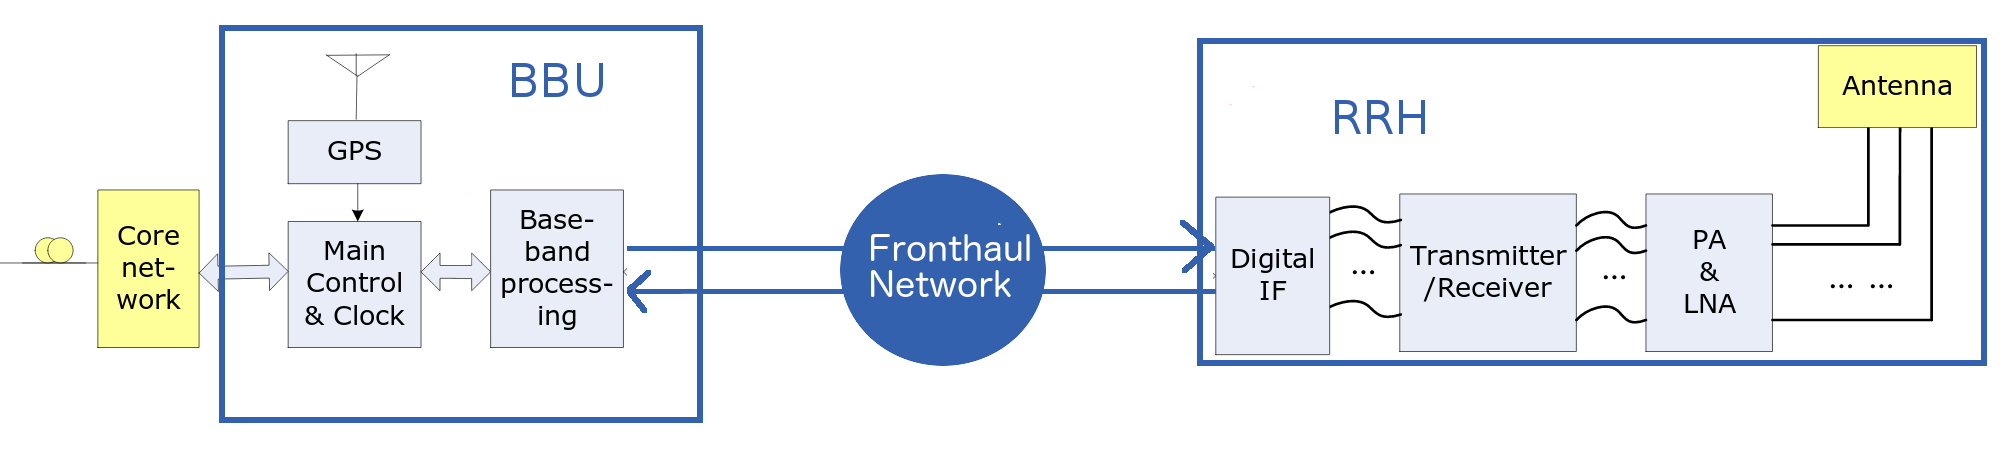
\includegraphics[scale=0.15]{BBURRH2.png}

    
\begin{itemize}
\item Contention in the fronthaul network
\item Need to guarantee the latency
\end{itemize}
 \end{center}
 
 \end{block}

 
 \end{frame}

 \begin{frame}
 \begin{center}
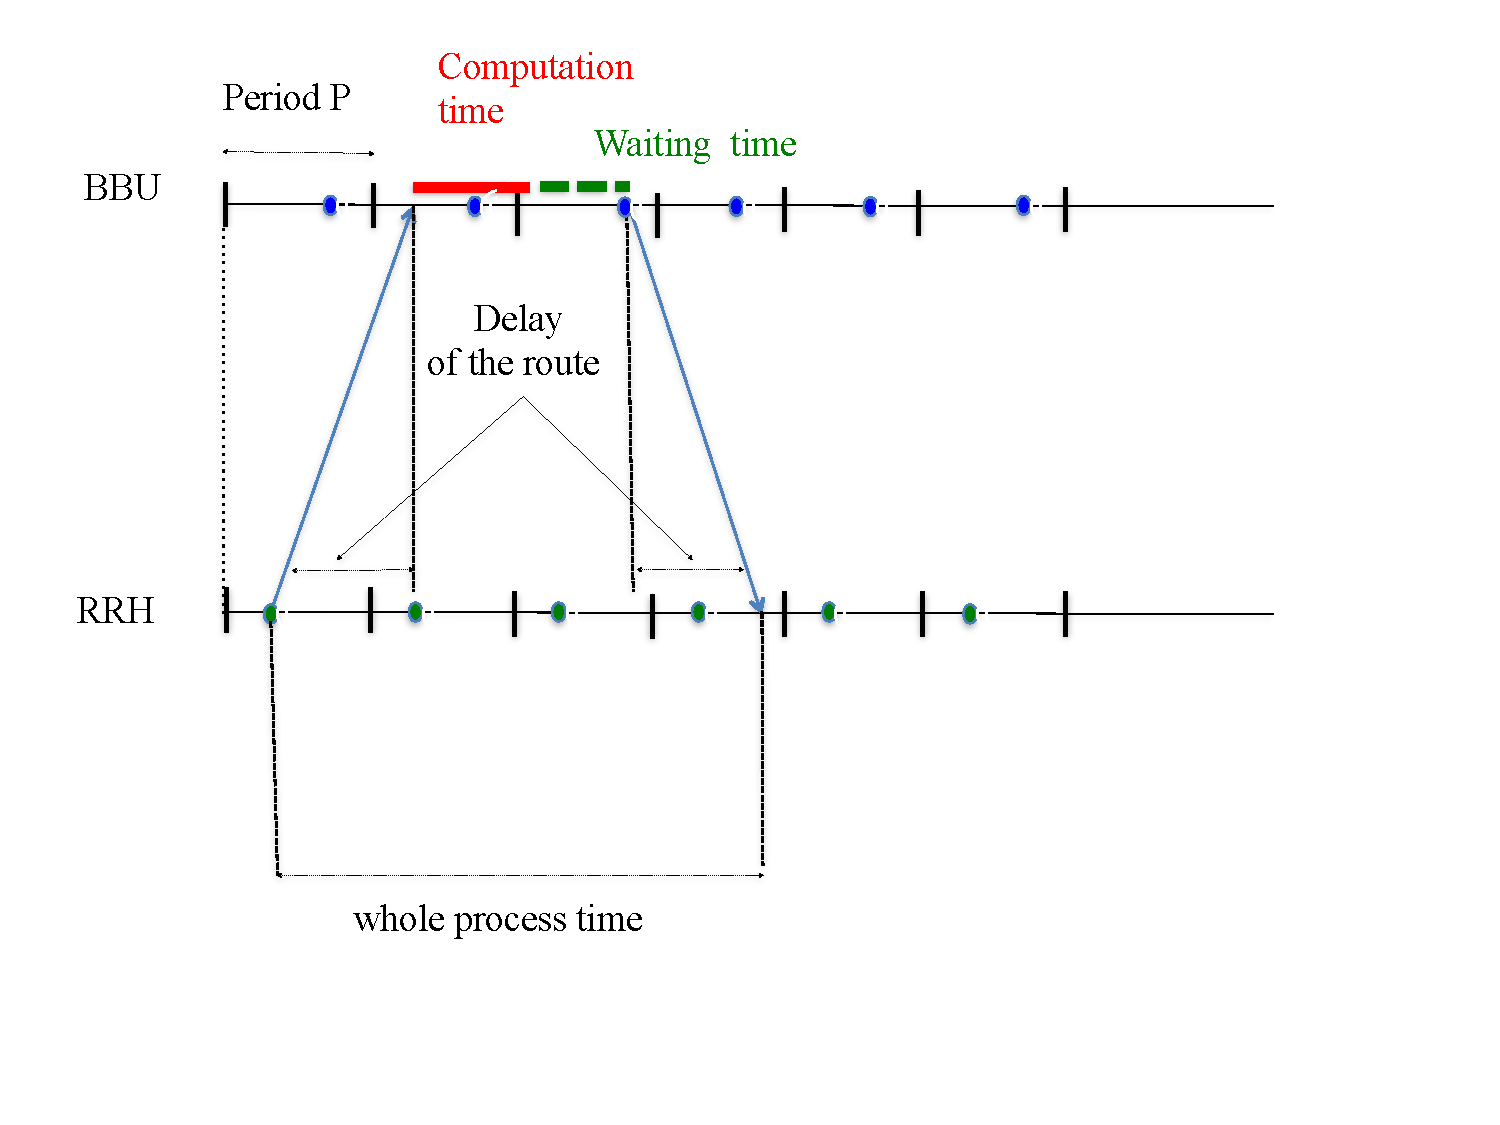
\includegraphics[scale=0.5]{periodic_process.pdf}

\end{center}
 \end{frame}


\begin{frame}{Model}

\centering
\scalebox{0.4}{

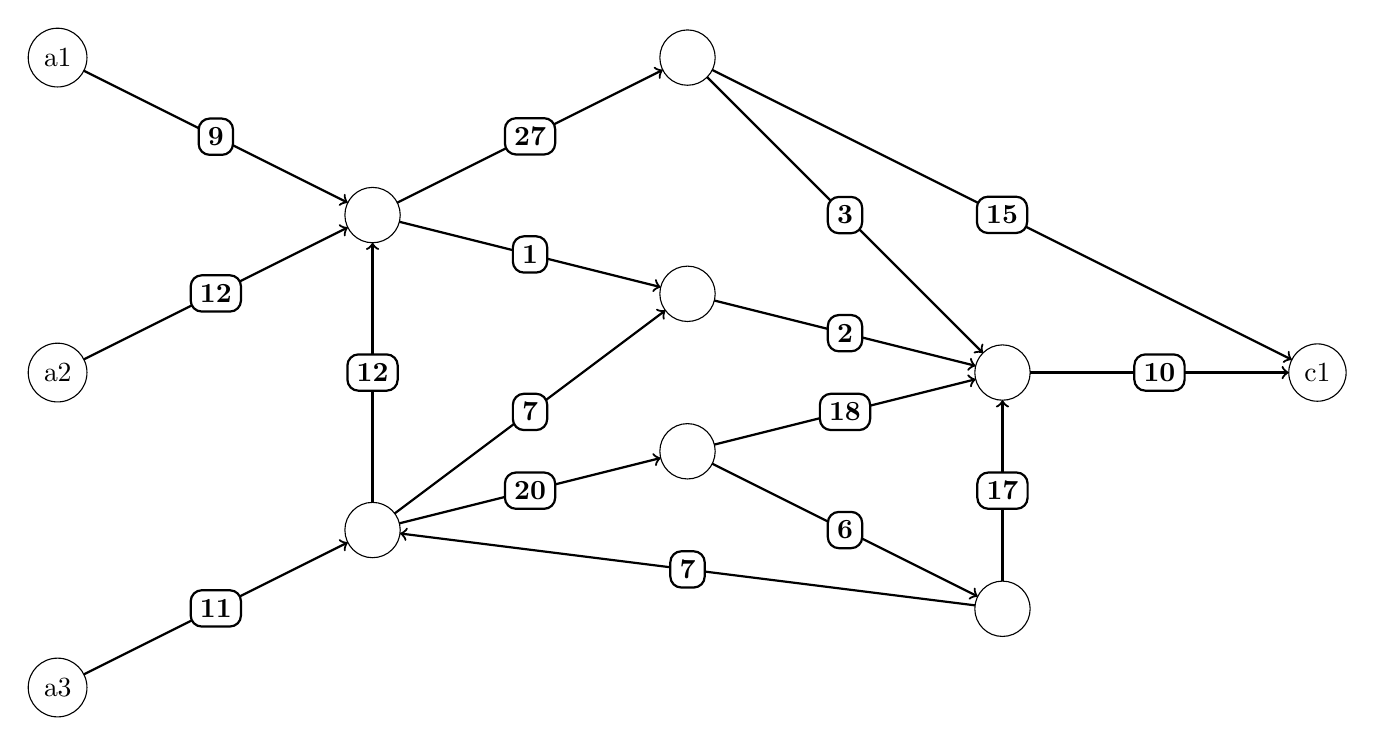
\begin{tikzpicture}
  \SetGraphUnit{5}
    \tikzset{
  EdgeStyle/.append style = {->} }
   \tikzstyle{VertexStyle}=[shape = circle, draw, minimum size = 20pt]
  \Vertex[x=0,y=0]{a3}
  \Vertex[x=0,y=4]{a2}
  \Vertex[x=0,y=8]{a1}


  \Vertex[x=16,y=4]{c1}
  
 \SetVertexNoLabel
  \Vertex[x=4,y=2]{n1}
  \Vertex[x=4,y=6]{n2}  
  \Vertex[x=12,y=1]{n3}
  \Vertex[x=12,y=4]{n4}
  \Vertex[x=8,y=3]{n6}
  \Vertex[x=8,y=5]{n7}
  \Vertex[x=8,y=8]{n8}



  \Edge[label = 12](n1)(n2)
  \Edge[label = 7](n3)(n1)
  \Edge[label = 3](n8)(n4)
  \Edge[label = 15](n8)(c1)
  \Edge[label = 27](n2)(n8)
  \Edge[label = 17](n3)(n4)
  \Edge[label = 7](n1)(n7)
  \Edge[label = 6](n6)(n3)
  \Edge[label = 9](a1)(n2)   
  \Edge[label = 2](n7)(n4)
  \Edge[label = 11](a3)(n1)
  \Edge[label = 20](n1)(n6)
  \Edge[label = 18](n6)(n4)
  \Edge[label = 12](a2)(n2)
  \Edge[label = 10](n4)(c1)
  \Edge[label = 1](n2)(n7)

 
\end{tikzpicture}
}
\vspace{1cm}
\begin{itemize}
\item Network : Directed Graph
\item RRH / BBU $\rightarrow$ set of vertices A (Antennas) and C (Computation)
\item  Physical Delay of a link $\rightarrow$ Weight on arcs
\end{itemize}

 \end{frame}
 


\begin{frame}{Model}
 \begin{block}{Slotted time}
  The time is discrete.
  \begin{itemize}
   \item Slot $\rightarrow$ 1$\mu$s.
   \item Step by step.
  \end{itemize}
 \end{block}


  \begin{block}{Message sending}


\centering
\scalebox{0.3}{

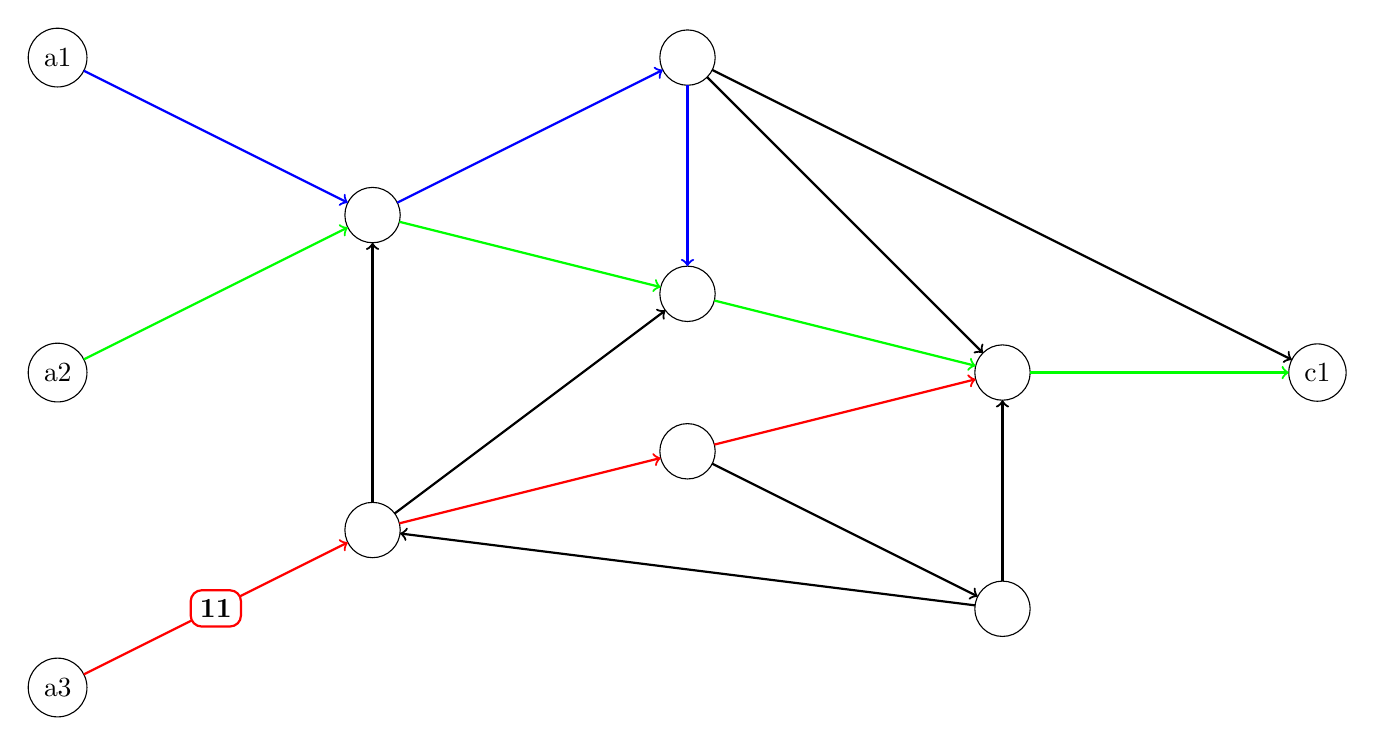
\begin{tikzpicture}
  \SetGraphUnit{5}
    \tikzset{
  EdgeStyle/.append style = {->} }
   \tikzstyle{VertexStyle}=[shape = circle, draw, minimum size = 20pt]
  \Vertex[x=0,y=0]{a3}
  \Vertex[x=0,y=4]{a2}
  \Vertex[x=0,y=8]{a1}


  \Vertex[x=16,y=4]{c1}
  
 \SetVertexNoLabel
  \Vertex[x=4,y=2]{n1}
  \Vertex[x=4,y=6]{n2}  
  \Vertex[x=12,y=1]{n3}
  \Vertex[x=12,y=4]{n4}
  \Vertex[x=8,y=3]{n6}
  \Vertex[x=8,y=5]{n7}
  \Vertex[x=8,y=8]{n8}



  \Edge(n1)(n2)
  \Edge(n3)(n1)
  \Edge(n8)(n4)
  \Edge(n8)(c1)

    \Edge(n3)(n4)
  \Edge(n1)(n7)
   

  \Edge(n6)(n3)

  
  \tikzset{
  EdgeStyle/.append style = {blue} }
  \Edge(a1)(n2)

  \Edge(n8)(n7)
   
  \Edge(n2)(n8)
   \tikzset{
  EdgeStyle/.append style = {red} }
    \Edge[label = 11](a3)(n1)

     \Edge(n1)(n6)
    \Edge(n6)(n4)

       \tikzset{
  EdgeStyle/.append style = {green} }
   \Edge(a2)(n2)
  \Edge(n4)(c1)
  \Edge(n2)(n7)
    \Edge(n7)(n4)
 
\end{tikzpicture}
}

Block of one or several slots used by the messages.
 \end{block}

\end{frame}

\begin{frame}{Latency}
 \begin{block}{Latency}
 3 factors increases the latency
 \begin{enumerate}
 \item The physical delay of the links (not alterable).
 \item The time before inserting a messages in the network.
 \item The buffering time of the messages in the network.
 \end{enumerate}
\end{block}

  \begin{block}{Collisions}


\centering
\scalebox{0.3}{

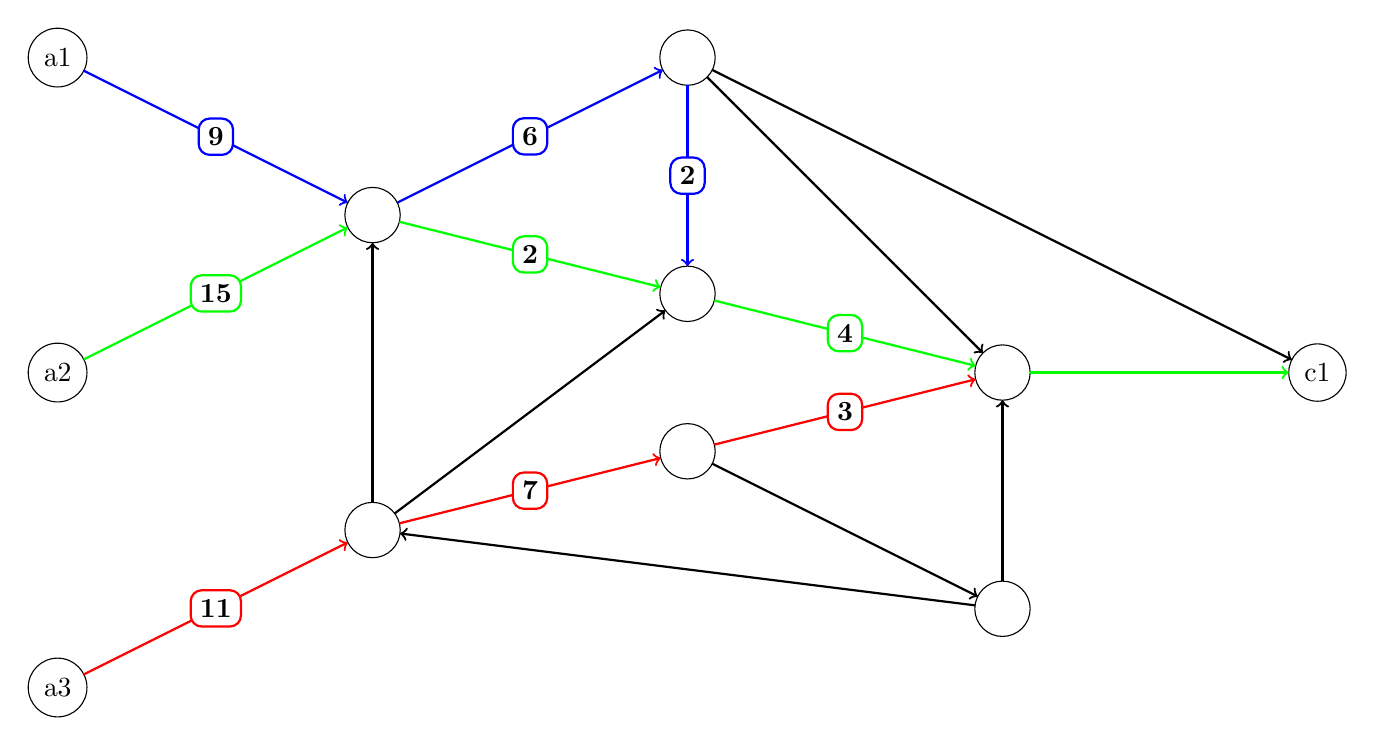
\begin{tikzpicture}
  \SetGraphUnit{5}
    \tikzset{
  EdgeStyle/.append style = {->} }
   \tikzstyle{VertexStyle}=[shape = circle, draw, minimum size = 20pt]
  \Vertex[x=0,y=0]{a3}
  \Vertex[x=0,y=4]{a2}
  \Vertex[x=0,y=8]{a1}


  \Vertex[x=16,y=4]{c1}
  
 \SetVertexNoLabel
  \Vertex[x=4,y=2]{n1}
  \Vertex[x=4,y=6]{n2}  
  \Vertex[x=12,y=1]{n3}
  \Vertex[x=12,y=4]{n4}
  \Vertex[x=8,y=3]{n6}
  \Vertex[x=8,y=5]{n7}
  \Vertex[x=8,y=8]{n8}



  \Edge(n1)(n2)
  \Edge(n3)(n1)
  
  \Edge(n8)(c1)
  \Edge(n1)(n7)
    \Edge(n3)(n4)


  \Edge(n6)(n3)
\Edge(n8)(n4)
  
  \tikzset{
  EdgeStyle/.append style = {blue} }
  \Edge[label = 9](a1)(n2)
\Edge[label = 2](n8)(n7)
     \Edge[label = 6](n2)(n8)
   

   \tikzset{
  EdgeStyle/.append style = {red} }
    \Edge[label = 11](a3)(n1)

     \Edge[label = 7](n1)(n6)
    \Edge[label = 3](n6)(n4)

       \tikzset{
  EdgeStyle/.append style = {green} }
   \Edge[label = 15](a2)(n2)
  \Edge(n4)(c1)
  \Edge[label = 2](n2)(n7)
     \Edge[label = 4](n7)(n4)

\end{tikzpicture}
}
 \end{block}


\end{frame}



  
  \begin{frame}{An easy topology}
  
  \centering

Control of the contention : reserving slots on routes.
\vspace{1cm}

\begin{block}{Star network}
  \centering
\scalebox{0.4}{
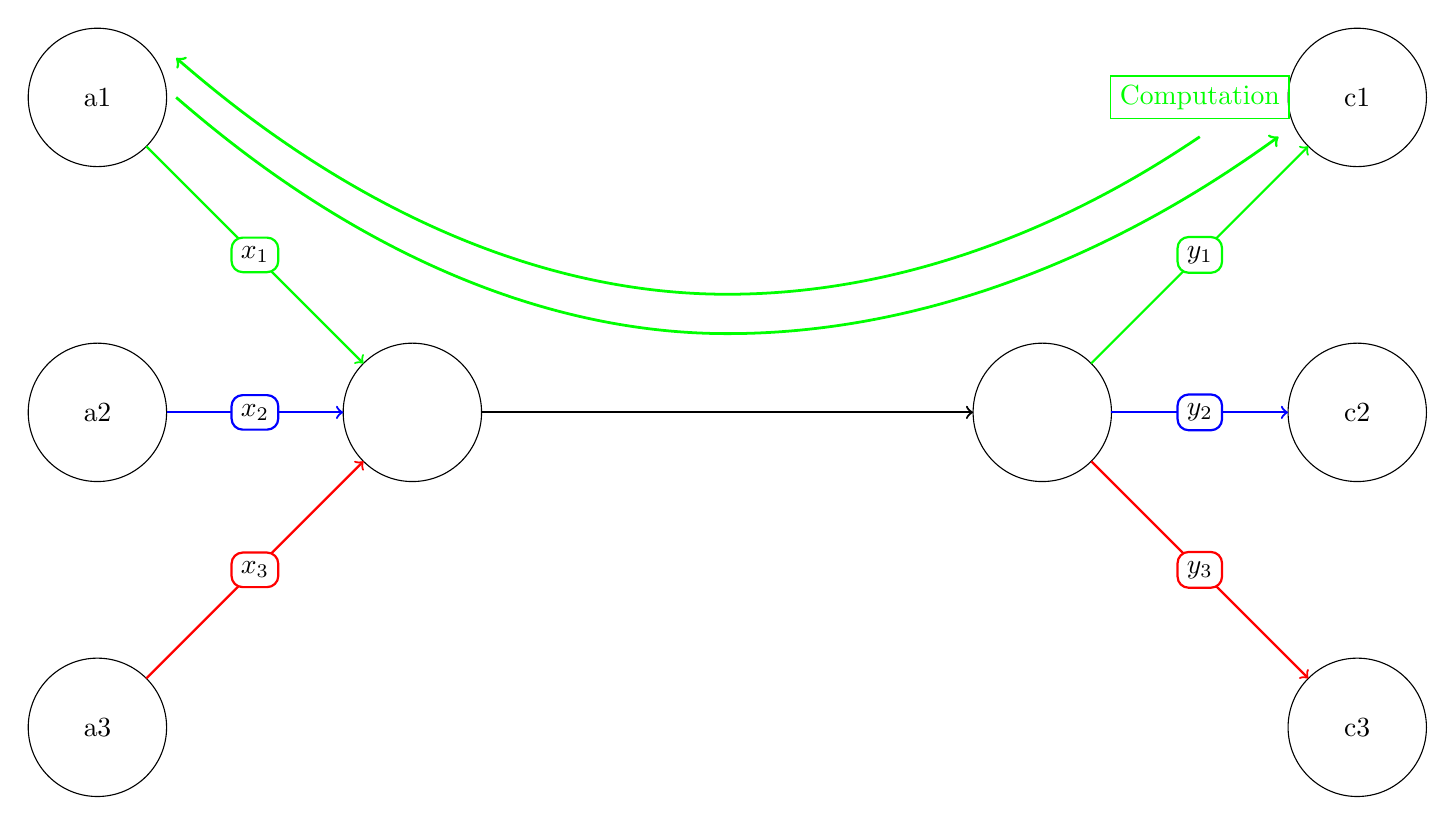
\begin{tikzpicture}
    \SetGraphUnit{5}
  \tikzstyle{VertexStyle}=[shape = circle, draw, minimum size = 50pt]
  \Vertex[x=0,y=0]{a3}
  \Vertex[x=0,y=4]{a2}
  \Vertex[x=0,y=8]{a1}
  
  \Vertex[x=16,y=0]{c3}
  \Vertex[x=16,y=4]{c2}
  \Vertex[x=16,y=8]{c1}
  
  \SetVertexNoLabel
  \Vertex[x=4,y=4]{SL}
  \Vertex[x=12,y=4]{SS}  
  \tikzset{
  EdgeStyle/.append style = {<-,green} }
  \Edge[label = $y_1$](c1)(SS)
  \Edge[label = $x_1$](SL)(a1)
  
  \tikzset{
  EdgeStyle/.append style = {blue} }
  \Edge[label = $y_2$](c2)(SS)
  \Edge[label = $x_2$](SL)(a2)
  
  \tikzset{
  EdgeStyle/.append style = {red} }
  \Edge[label = $y_3$](c3)(SS)
  \Edge[label = $x_3$](SL)(a3)
  
  \tikzset{
  EdgeStyle/.append style = {black} }
  \Edge(SS)(SL)
  
  \draw[->,line width=1pt,green] (1,8) parabola bend (8,5) (15,7.5);
  \node[draw,green] at (14,8) {Computation};
  \draw[<-,line width=1pt,green] (1,8.5) parabola bend (8,5.5) (14,7.5);


\end{tikzpicture}
}
\end{block}

\end{frame}

\begin{frame}{Problem}

\begin{block}{Problem}
Find some time at which send the messages from the BBU/RRH, such that there is no collisions in the network.
\end{block}
\vspace{1cm}
\begin{block}{\NP-hard}
On topology with restricted parameters.
\end{block}
\end{frame}

\begin{frame}{Main ideas}

\begin{block}{No buffering in BBU}
\begin{itemize}
\item Greedy Policy : ensure a solution for small loads
\item Shortest-Longest : ensure a solution for similar length of routes
\item Exhaustive search : optimal solutions for few routes
\end{itemize}

\end{block}

\begin{block}{Allowing buffers in BBU}
Two greedy parts: 

 \begin{multicols}{2}
 Way forward
\begin{itemize}
\item Multiple random sendings
\end{itemize}
\vspace{0.5cm}
Way backward
\begin{itemize}
\item Greedy Algorithm
\item Adapted scheduling algorithm
\end{itemize}
\end{multicols}
\vspace{1cm}
\end{block}

\end{frame}

\begin{frame}{Deterministic vs Stochastic}
\centering
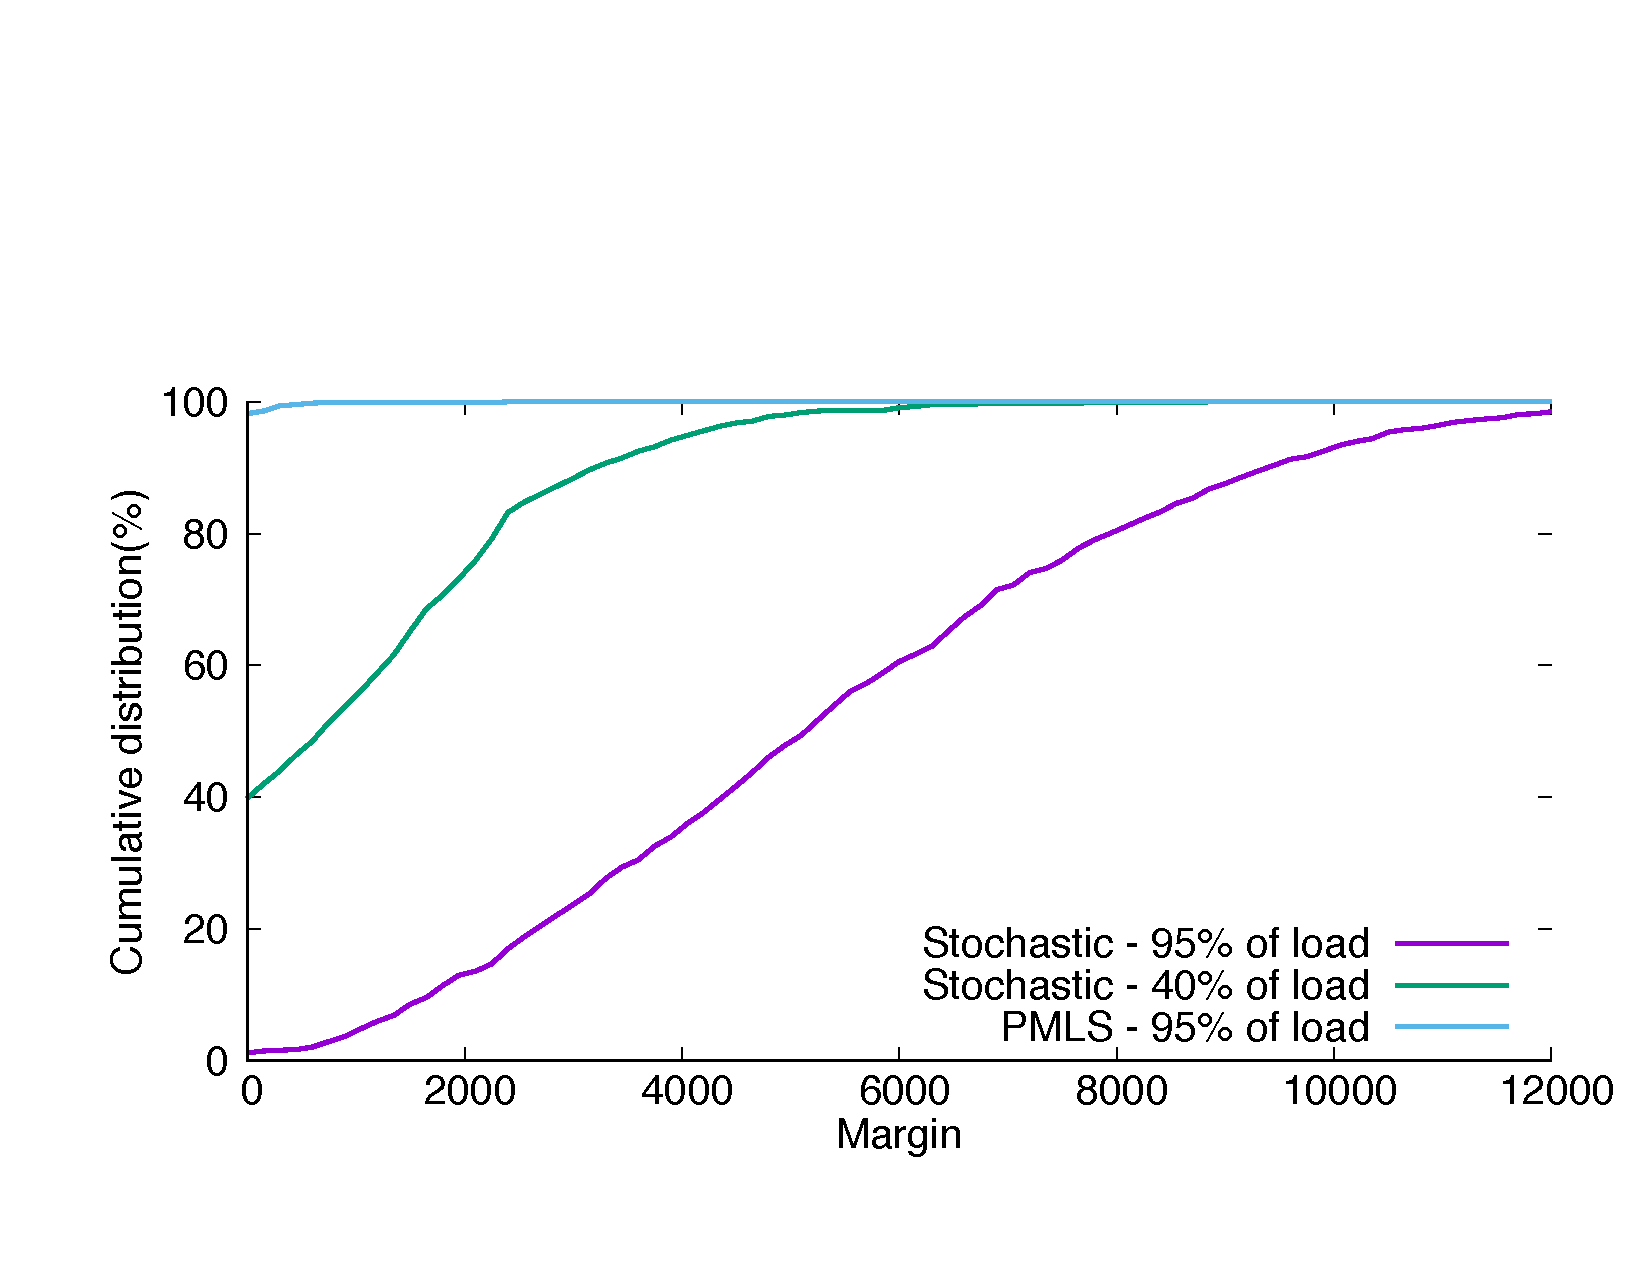
\includegraphics [width=100mm]{stochastic.pdf}
\end{frame}




\begin{frame}{Optical ring}




\begin{block}{Model}
\begin{center}
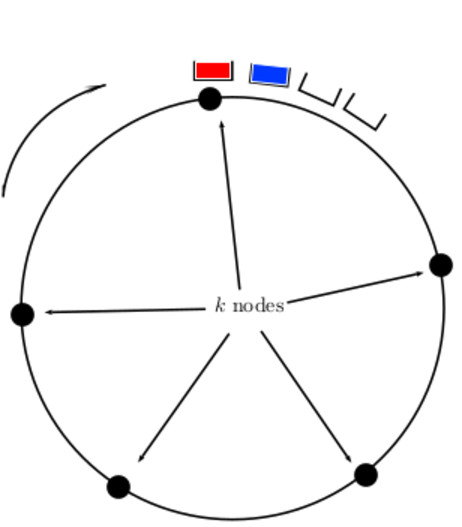
\includegraphics[scale=0.3]{anneau1.pdf}
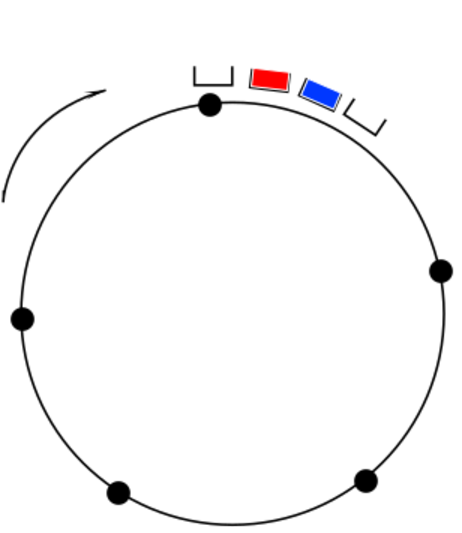
\includegraphics[scale=0.3]{anneau2.pdf}

Waiting only at the insertion
\end{center}
\end{block}

\begin{center}
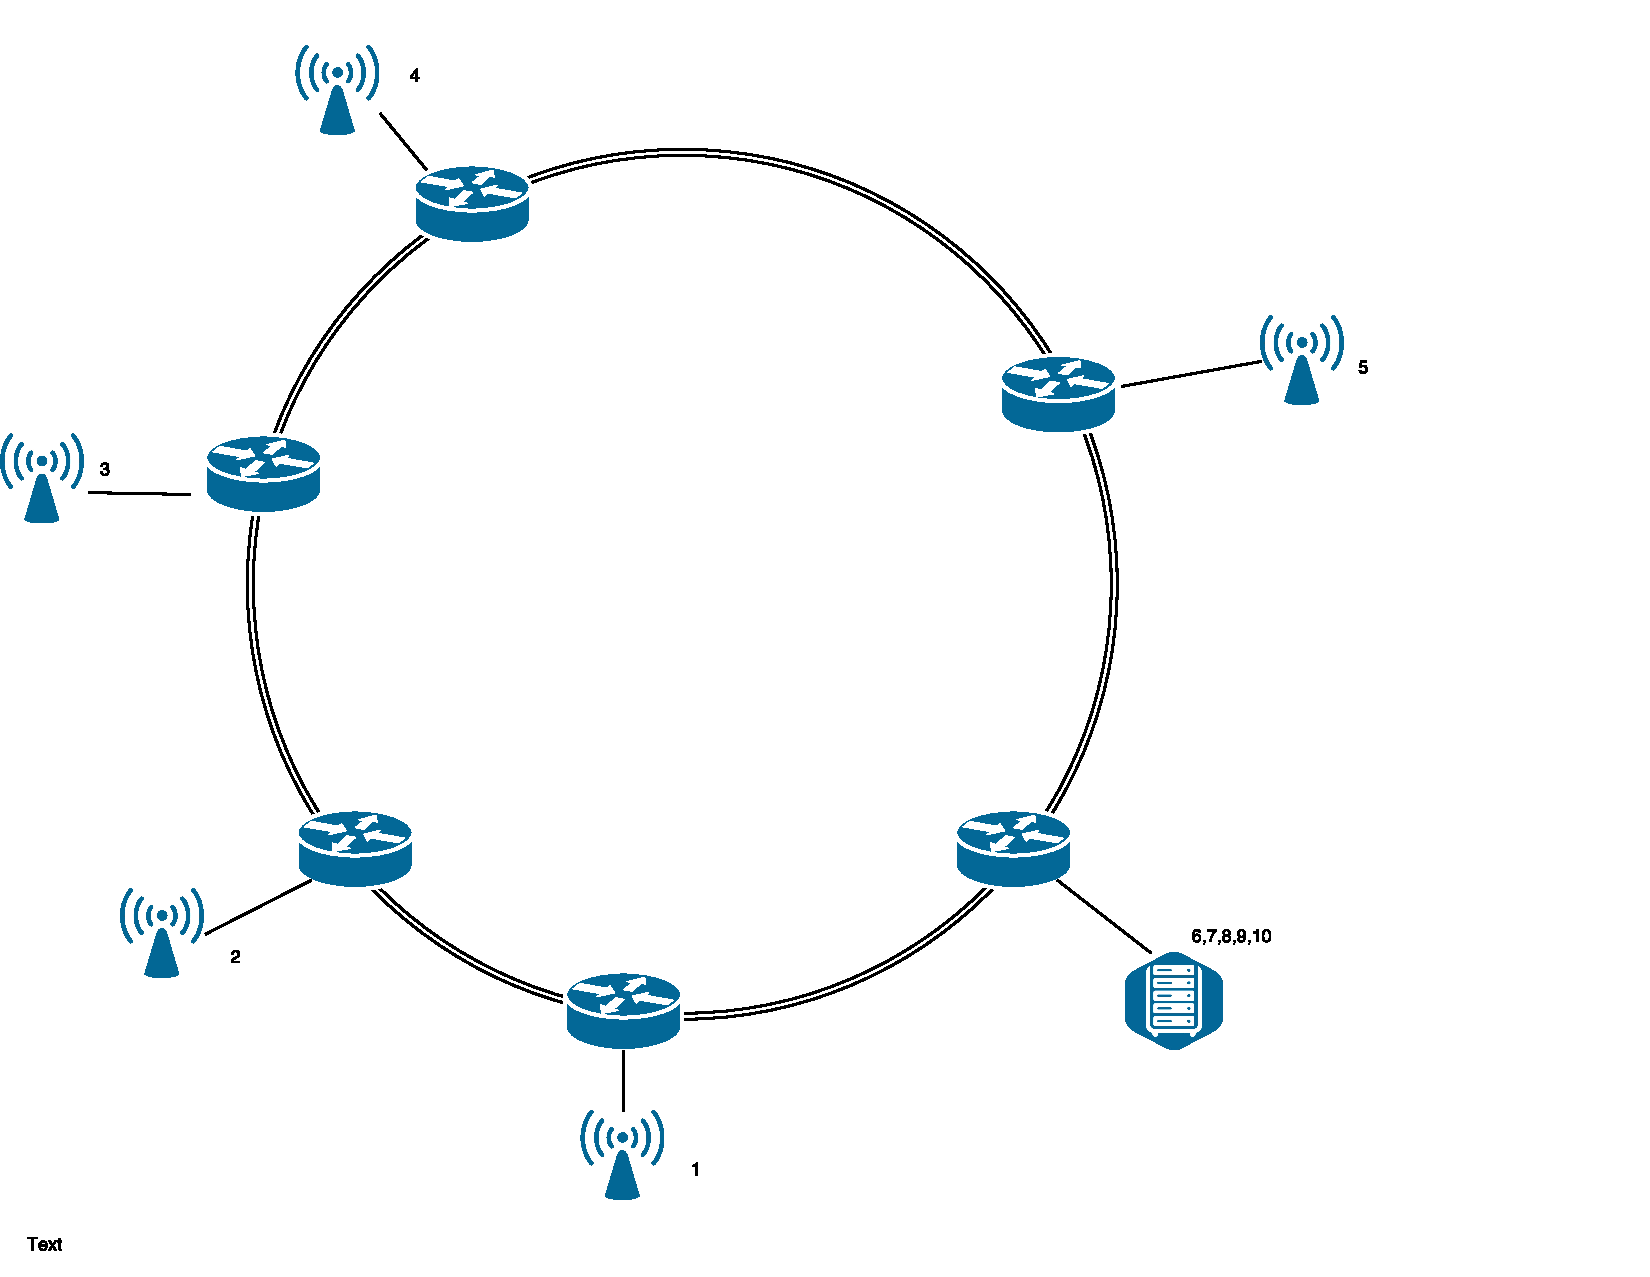
\includegraphics[scale=0.13]{anneau-simple.pdf}
\end{center}


\end{frame}


\begin{frame}{Insertion}


\begin{center}
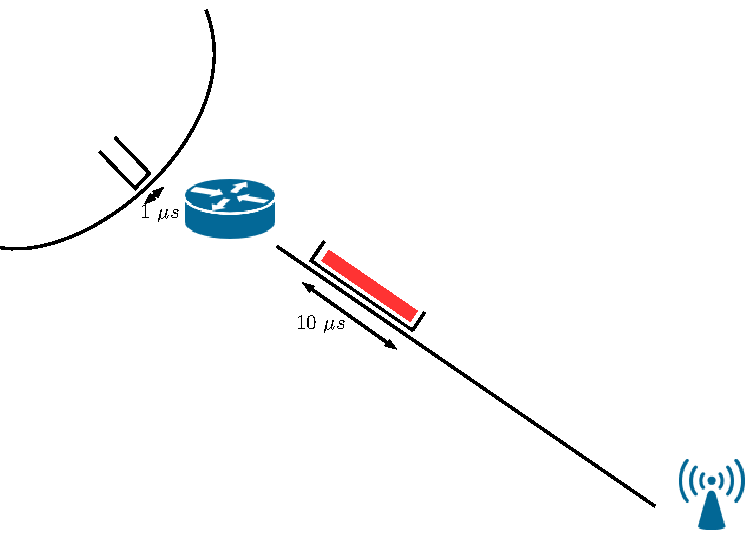
\includegraphics[scale=0.4]{slot1.pdf}
\hspace{1cm}
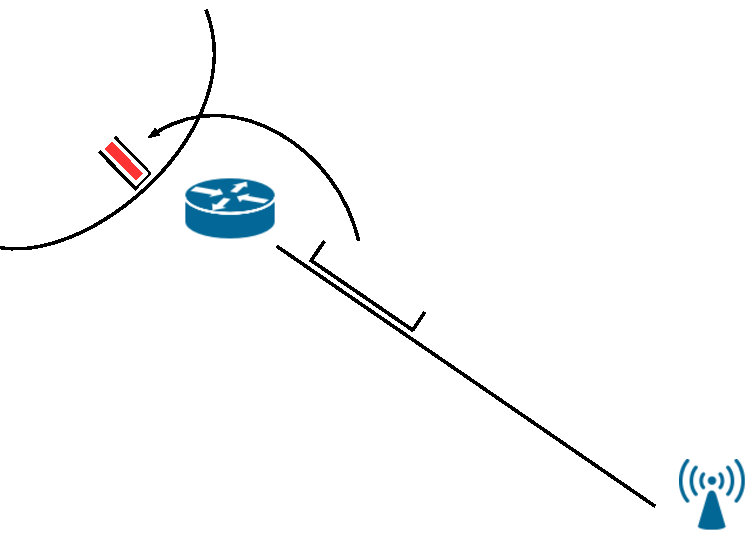
\includegraphics[scale=0.4]{slot2.pdf}

\end{center}

\end{frame}





\begin{frame}{Parameters}
 \centering Broadcast and select Policy 
 
 
 \begin{block}{Parameters}
\centering
  \begin{tabular}{|c|c|c|}
  \hline
  Length of the ring & 20km & 100 slots\\
   \hline
  Number of nodes & 3 -10 & \\
  \hline
  Duration of a slot & 1$\mu$s & -\\
  \hline
  Bandwidth & 100 Gbps & -\\
  \hline
    Period & 1ms & 1000 slots\\
  \hline
    Capacity of a packet & 1Mb & -\\
  \hline
      Flow of an antenna & 5Gbps & 1 packet/Every 10 slots during 500 slots\\
  \hline
  \end{tabular}

 \end{block}

\end{frame}

\begin{frame}{Optical ring problematic}
\begin{itemize}
\item We got two kinds of traffic : CRAN - high priority, Best effort
\vspace{1cm}
\item We want to observe the behavior of the ring and analyze the latency of CRAN
\vspace{1cm}
\item We will try to find some methods to decrease the CRAN latency without increasing the Best effort latency too much
\end{itemize}
\end{frame}

\begin{frame}{No management}

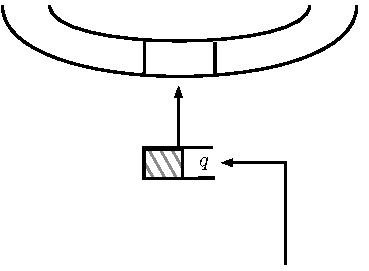
\includegraphics[width=0.5\textwidth]{insertion0.pdf}
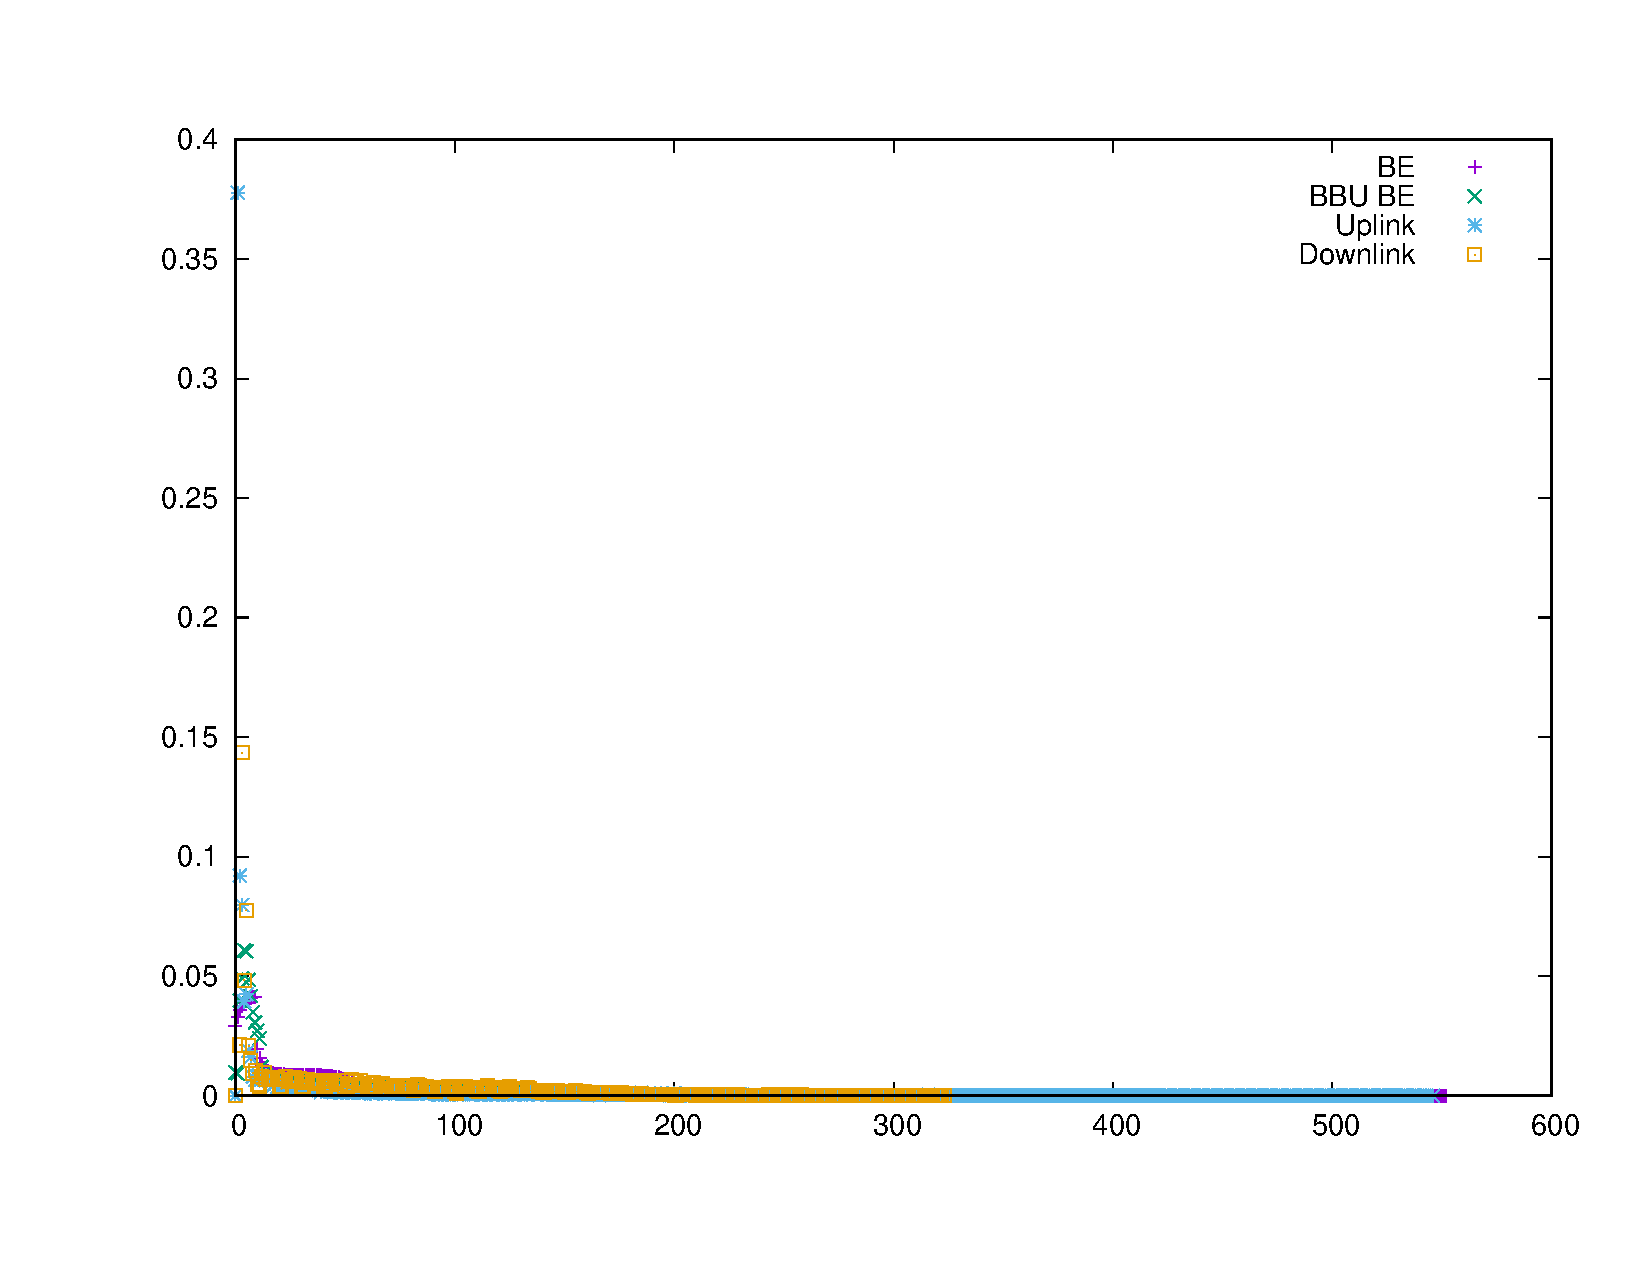
\includegraphics[width=0.5\textwidth]{No_managment_low.pdf}

\centering Average Load = 0.8

\end{frame}


\begin{frame}{Priority with low load}

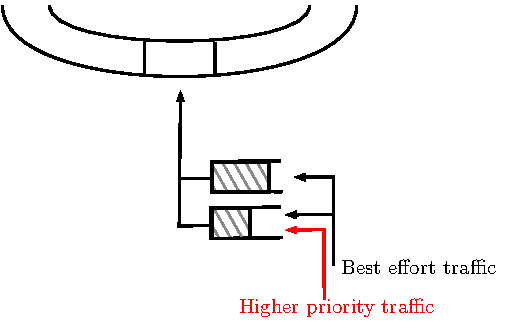
\includegraphics[width=0.5\textwidth]{insertion1.pdf}
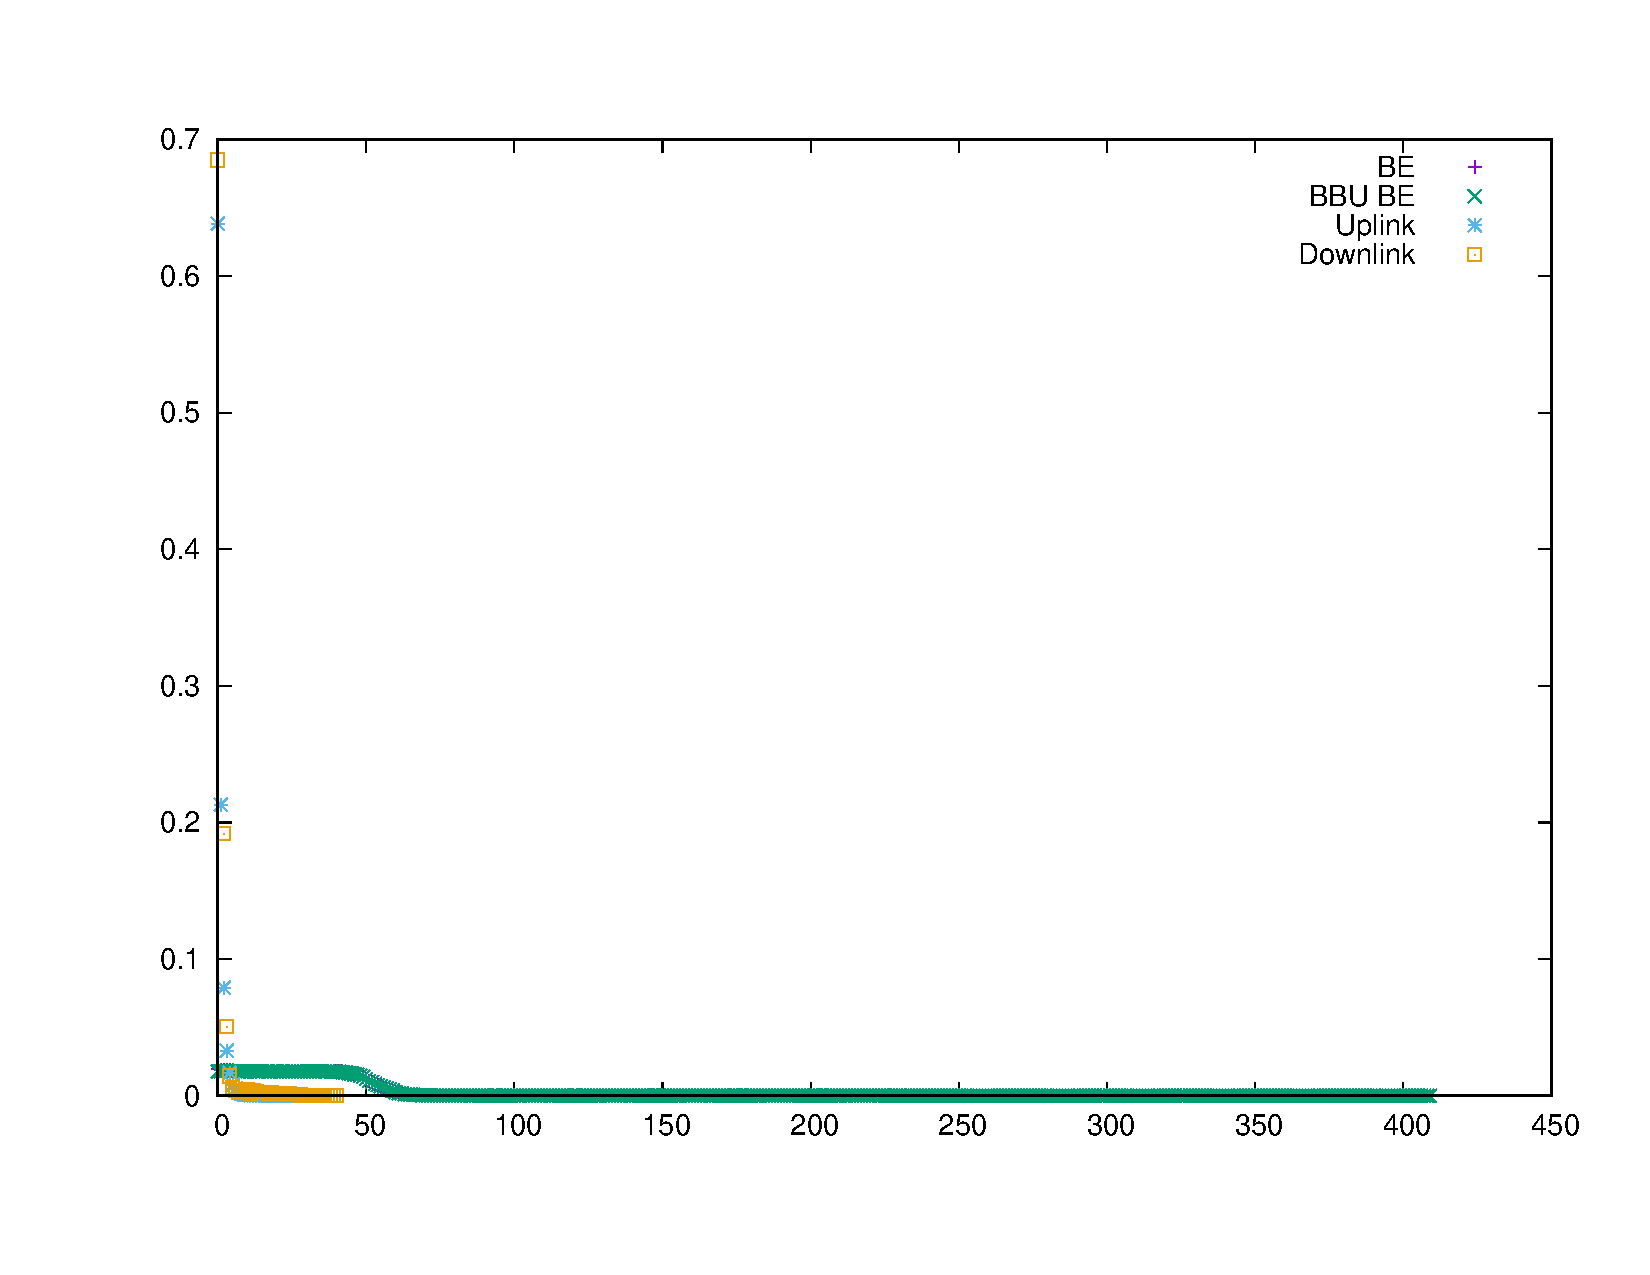
\includegraphics[width=0.5\textwidth]{Priority_low.pdf}

\centering Average Load = 0.58

\end{frame}

\begin{frame}{Priority with high load}


  \begin{textblock*}{120mm}(10mm,3cm) % {block width} (coords)
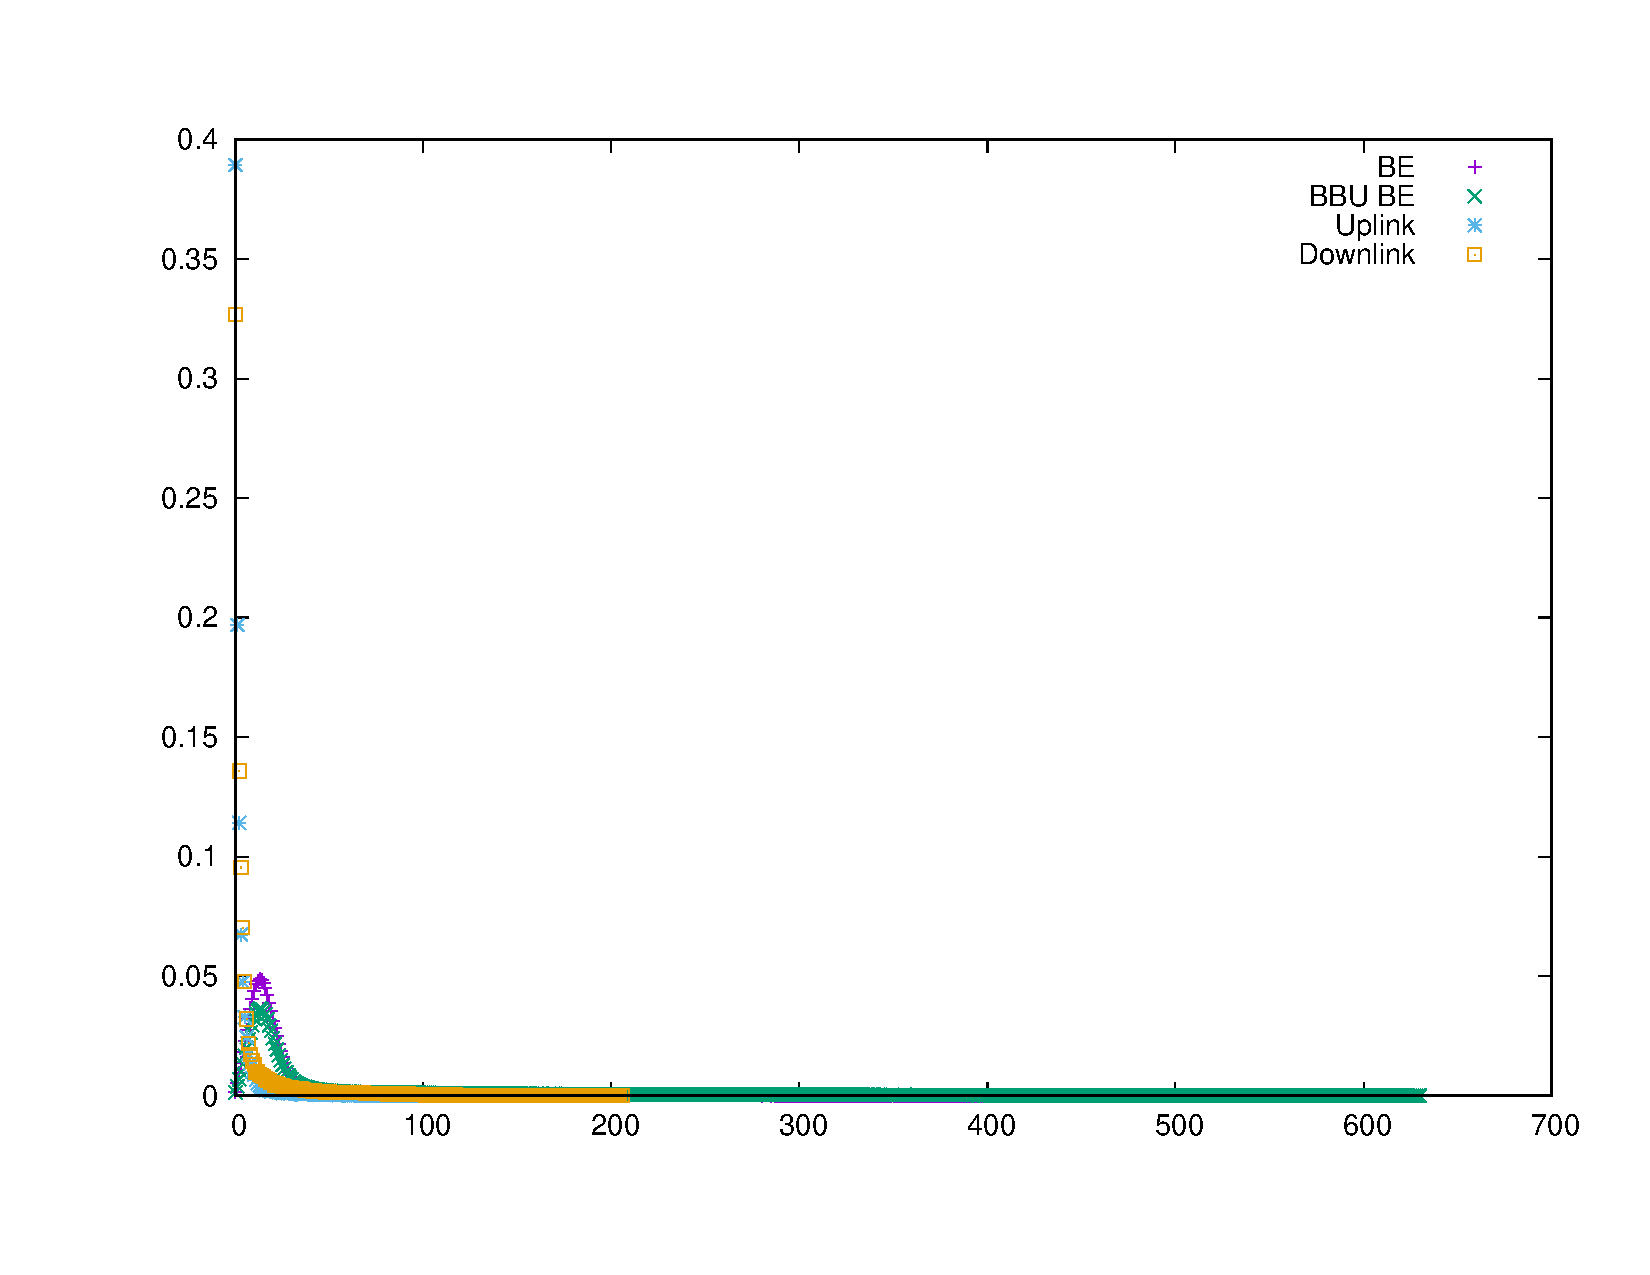
\includegraphics[width=0.5\textwidth]{Priority_high.pdf} 
\end{textblock*}


  \begin{textblock*}{100mm}(70mm,4cm) % {block width} (coords)
\begin{itemize}
\item Average load = 0.85
\item More BE than without priority 
\end{itemize}
\end{textblock*}
\end{frame}

\begin{frame}{Deterministic policy}

\hspace{2cm}
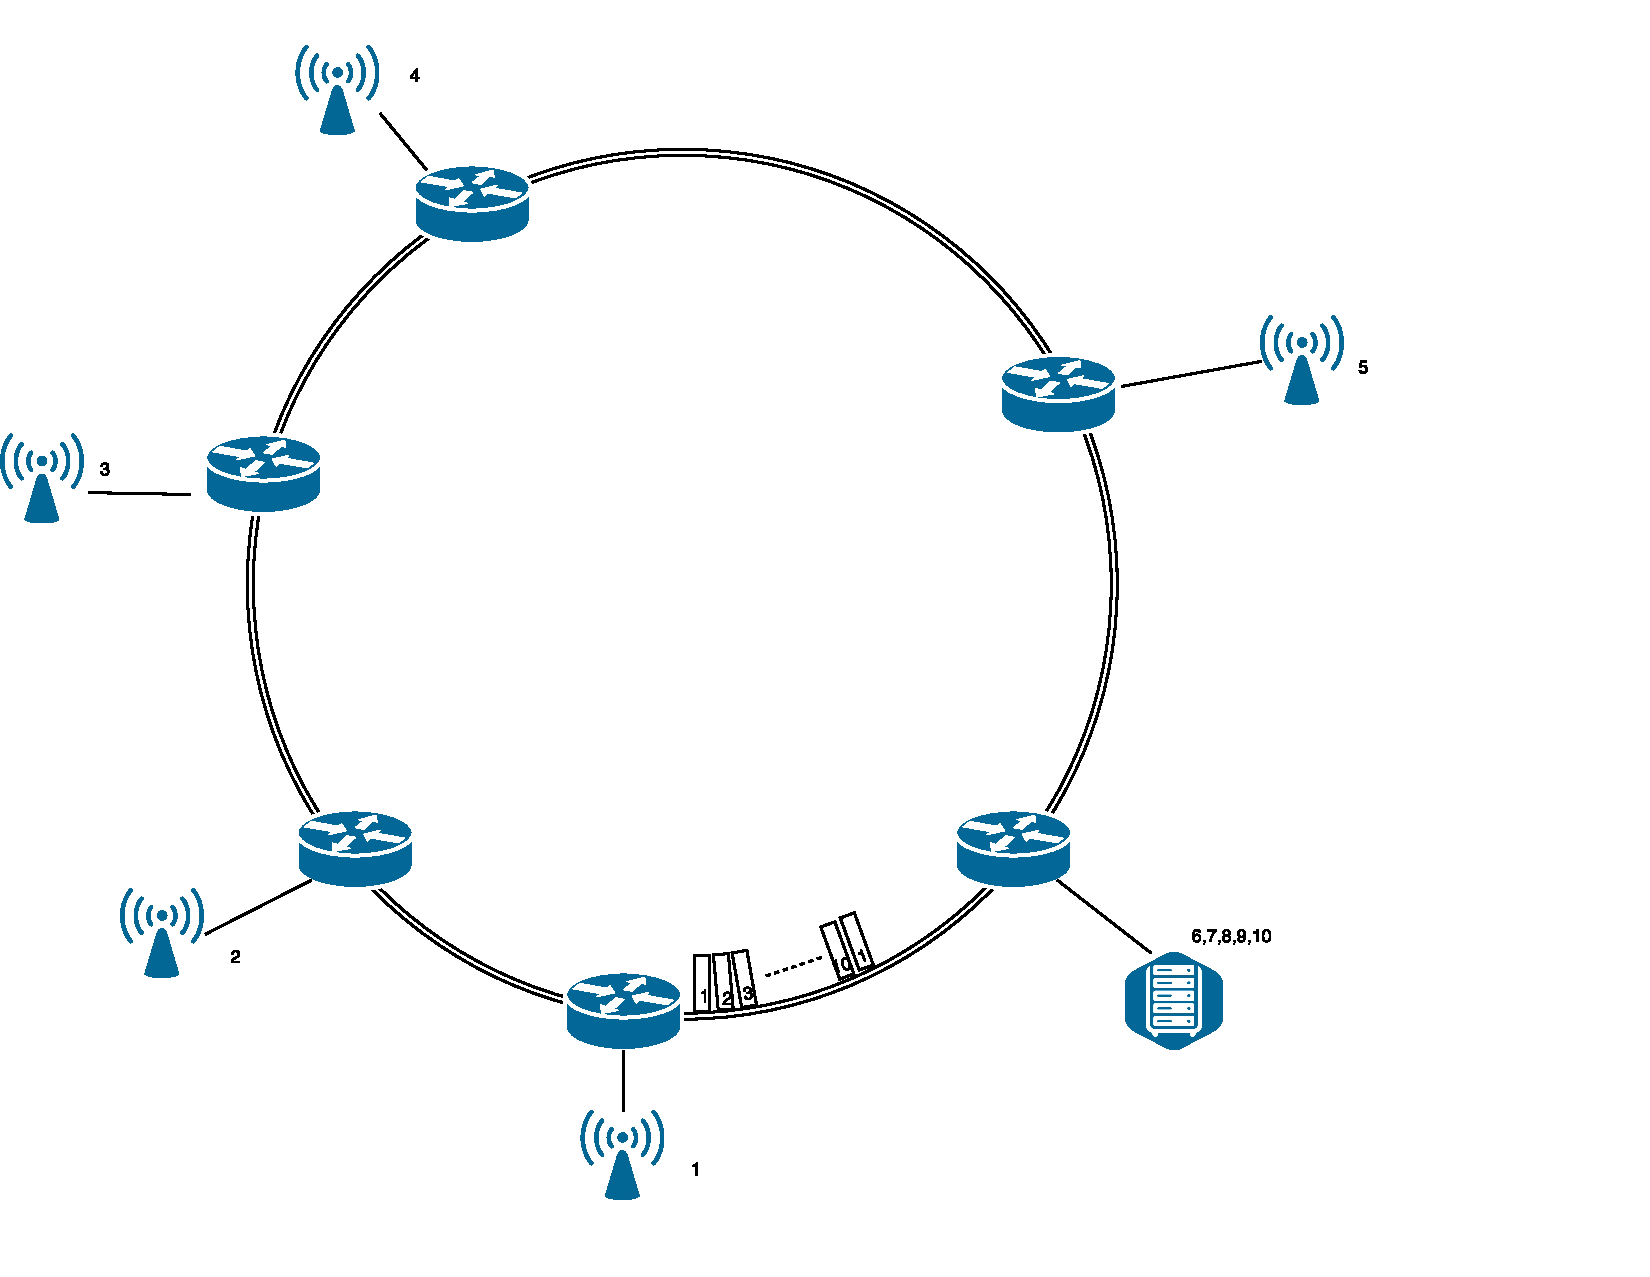
\includegraphics[scale=0.35]{slotsanneau.pdf}



\end{frame}




\begin{frame}{Rerservation}



\centering 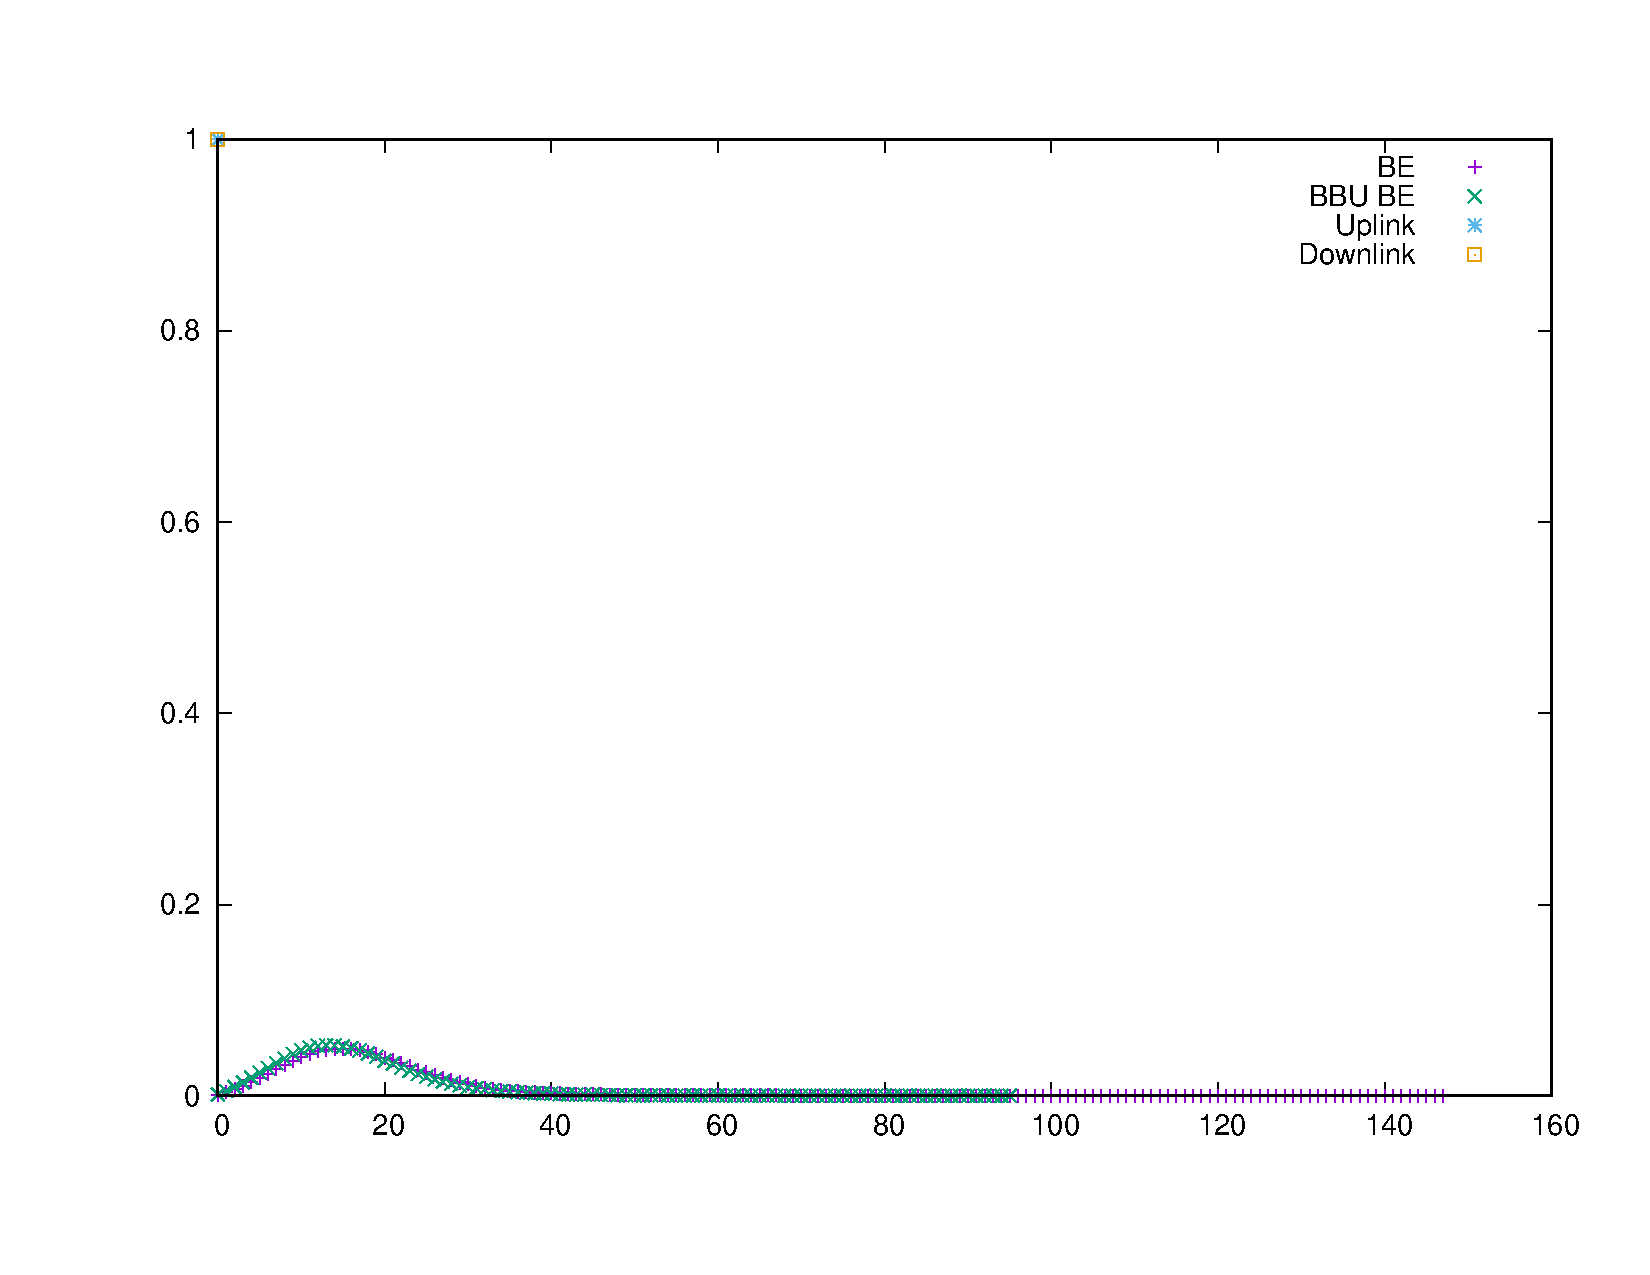
\includegraphics[width=0.7\textwidth]{Resa_high_1.pdf} 


\centering Loaded network

\end{frame}


\begin{frame}{An harder topology}


\hspace{2cm}
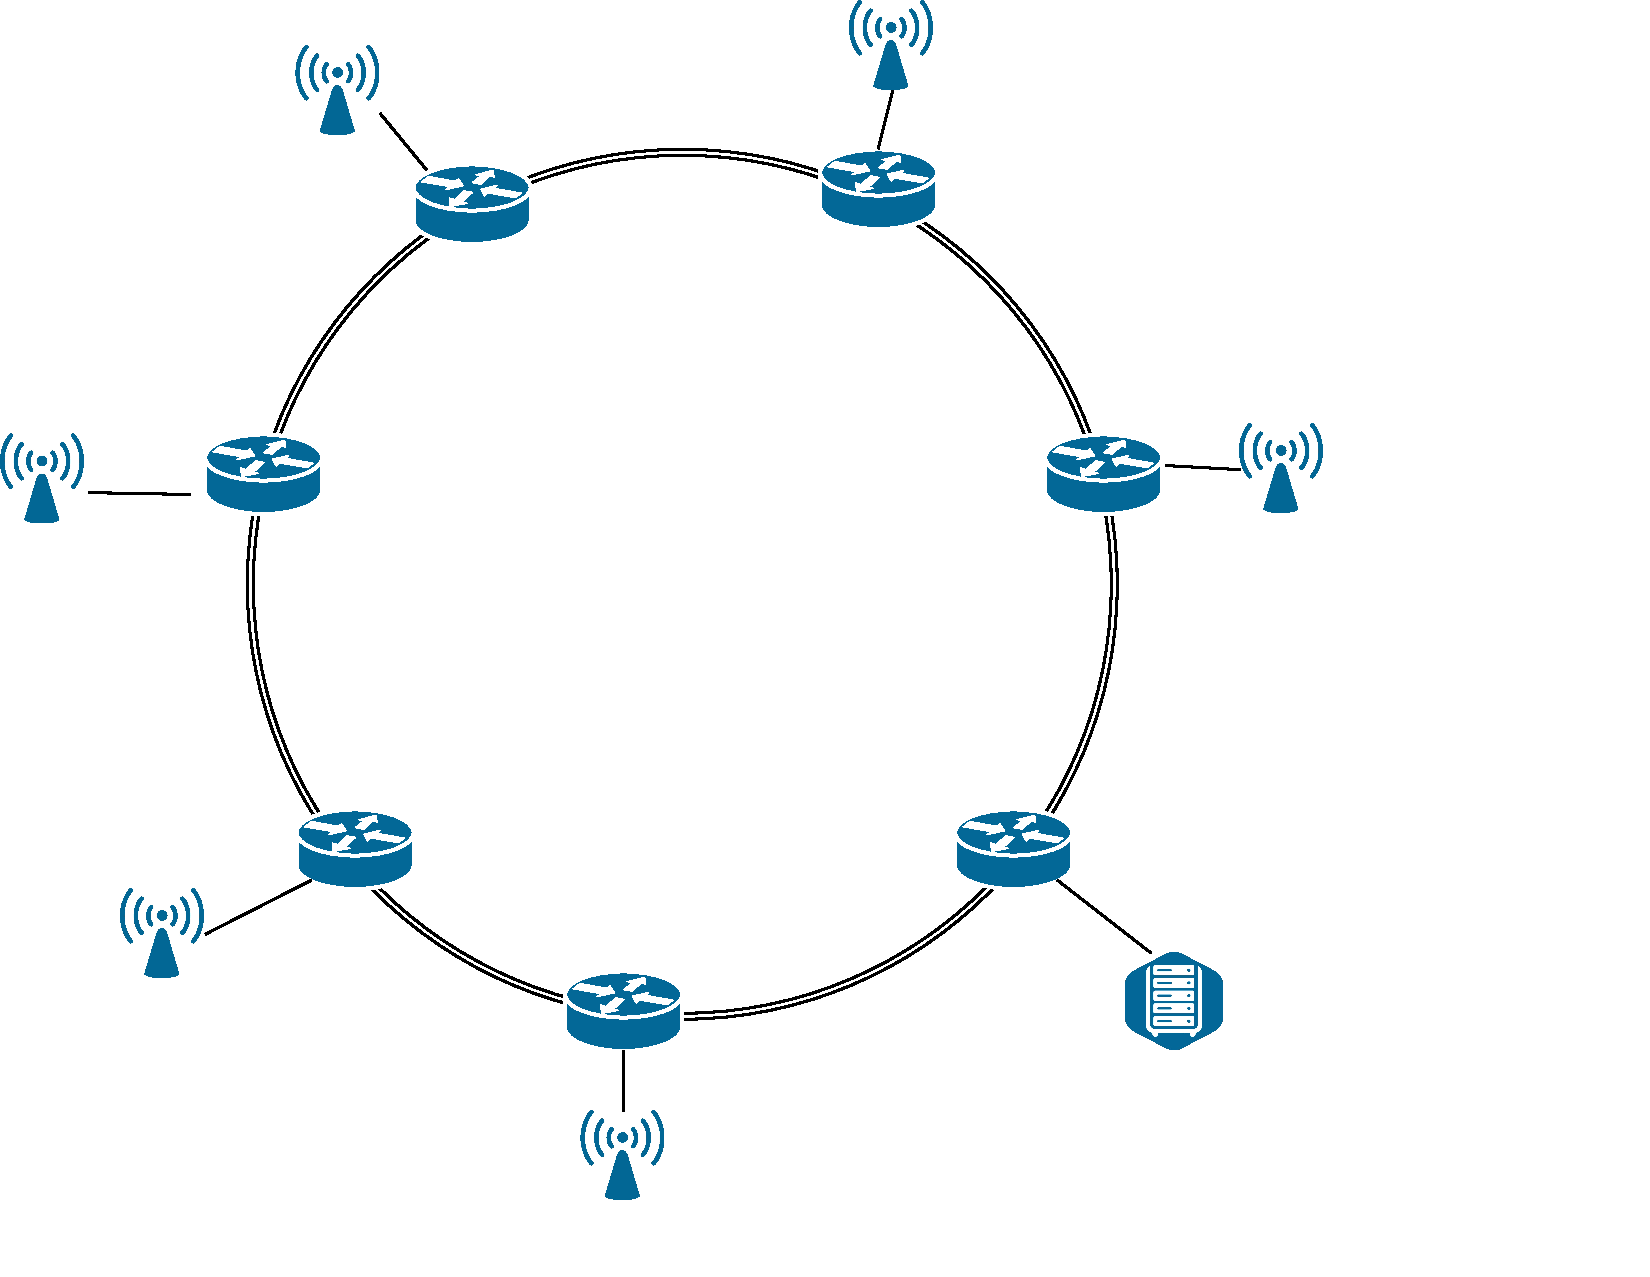
\includegraphics[scale=0.35]{anneau_probleme.pdf}


\end{frame}


\begin{frame}{Split frequencies}



\centering 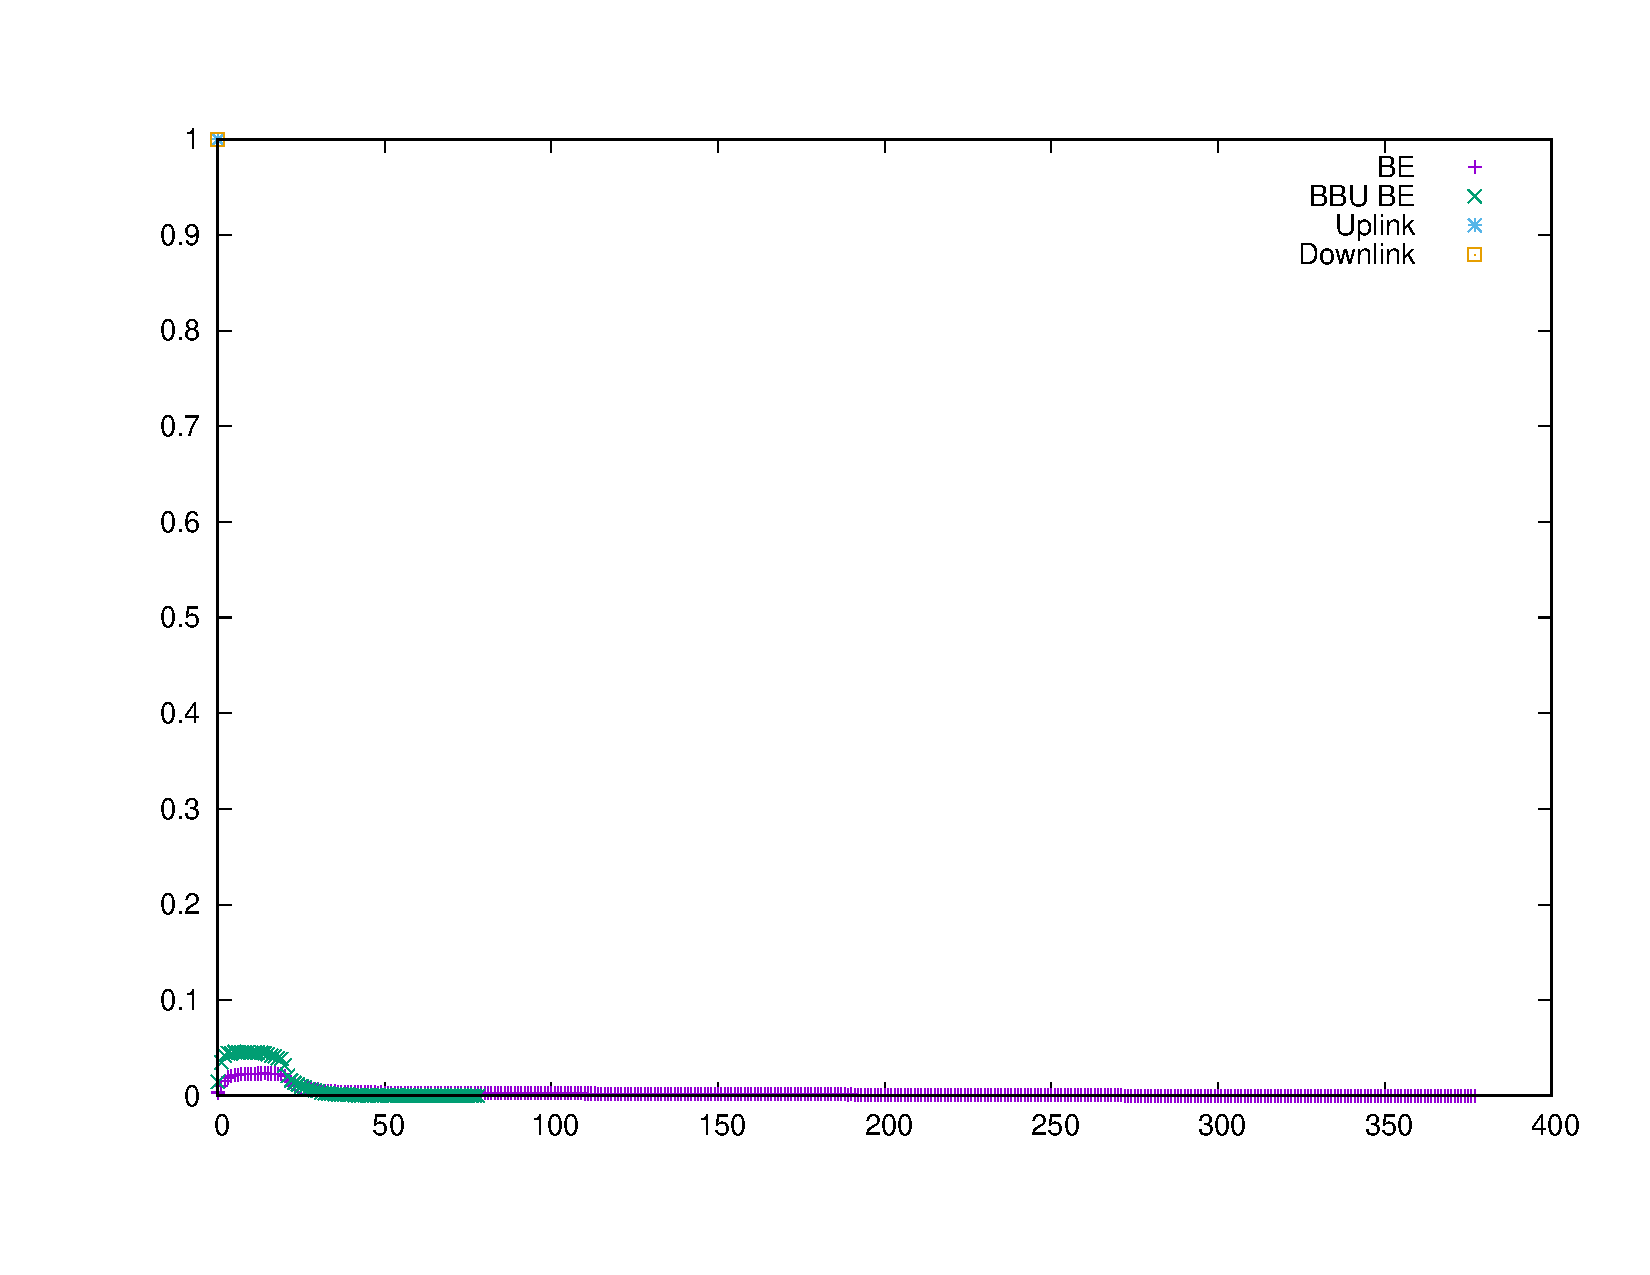
\includegraphics[width=0.7\textwidth]{Split_high.pdf} 

\centering 6 antennas/ less BE/ load increased 


\end{frame}







\begin{frame}{Future work}

\begin{enumerate}
\item Infocom review
\item Ngreen results 
\end{enumerate}
\end{frame}
\end{document}
